In this section we’ll discuss the results achieved from different experiments done on IP102 and D0.
\subsection{Evaluation Metrics}
The metrics used for different experiments we have done on the IP102 dataset will be explained here.
\subsubsection{Accuracy}
Accuracy denotes the ratio between all number of correct predictions and total number of predictions. Accuracy is calculated from the samples of the test dataset. The reason for choosing the test dataset is that the model didn’t have any glance over it during the training session. Thus, a better estimation can be achieved on the generalization capability of a model.
\begin{equation}
    Accuracy = \frac{M}{N}*100\%
\end{equation}
Here, M and N denote the number of samples for which the model could predict class labels accurately and the number of samples in the test set.
\subsubsection{Recall}
Recall, also known as sensitivity, is used in multiclass problems to evaluate the amount of correctly classified from the amount of samples which should have been identified as of that class. So, it’s a ratio of the true positive numbers of predictions, true positive predictions and false negative predictions among all the classes.\\
Recall for each class c is calculated by considering the one-vs-all strategy.
\begin{equation}
    \text{Recall, } c = \frac{TPc}{TPc+FNc}
\end{equation}
In the equation above, TPc denotes correctly classified samples numbers of c and FNc denotes the wrongly classified samples number of c.
For classes have imbalence problem, macro average recall is calculated where the recall is calculated for each class separately and their average is taken. This finally ensures that the model will be equally penalized for each false-negative instance of any class. For a set of classes C,
\begin{equation}
    \text{Macro Average Recall} = \frac{\Sigma_{i=0}^{n} \text{Recall}_i}{n}
\end{equation}
\subsubsection{Precision}
A model's precision is a metric for how correctly it can identify instances of a given class.
It is determined by dividing the total of true positive forecasts and false positive predictions by the number of true positive predictions, or predictions that are both accurate and for the target class (predictions that are correct for the target class but actually belong to another class).
Precision, also known as Positive Predictive Value, can be determined for each class in a multi-class issue by taking into account only the predictions made for that class (PPV). 
\begin{equation}
    Precision = \frac{TPc}{TPc + FPc}
\end{equation}
Here, the number of samples that are correctly identified as being in class c is known as true positive predictions (TPc), whereas the number of samples that are incorrectly identified as being in class c is known as false positive predictions (FPc).
Macro-average precision is frequently used to determine precision in datasets that are unbalanced, meaning that the classes are not distributed equally.
This entails determining precision for each class independently and averaging these results.
This makes sure that any incorrect positive prediction for any of the classes is penalized equally by the model.
The amount of true positive predictions and false positive predictions for each class should be taken into account while computing precision for a set of classes (C). 
\begin{equation}
    \text{Macro Average Precision} = \frac{\Sigma_{i=0}^{n} \text{Precision}_i}{n}
\end{equation}
Here, Precision is the precision value for class c, and \(|C|\) is the total number of classes.
\subsection{Class based analysis of IP102}
We trained the IP102 dataset with ResNet50, ResNet152 and ResNet18 and found insights on the dataset as summarized bellow-
\begin{itemize}
    \item Higher number of samples does not guarantee higher accuracy.
    \item Higher accuracy can be achieved from least number of samples. 
    \item Higher accuracy was achieved from comparatively complex images.
    \item Lower accuracy were shown from comparatively simple images.
\end{itemize}
\begin{sidewaysfigure}
    \centering
    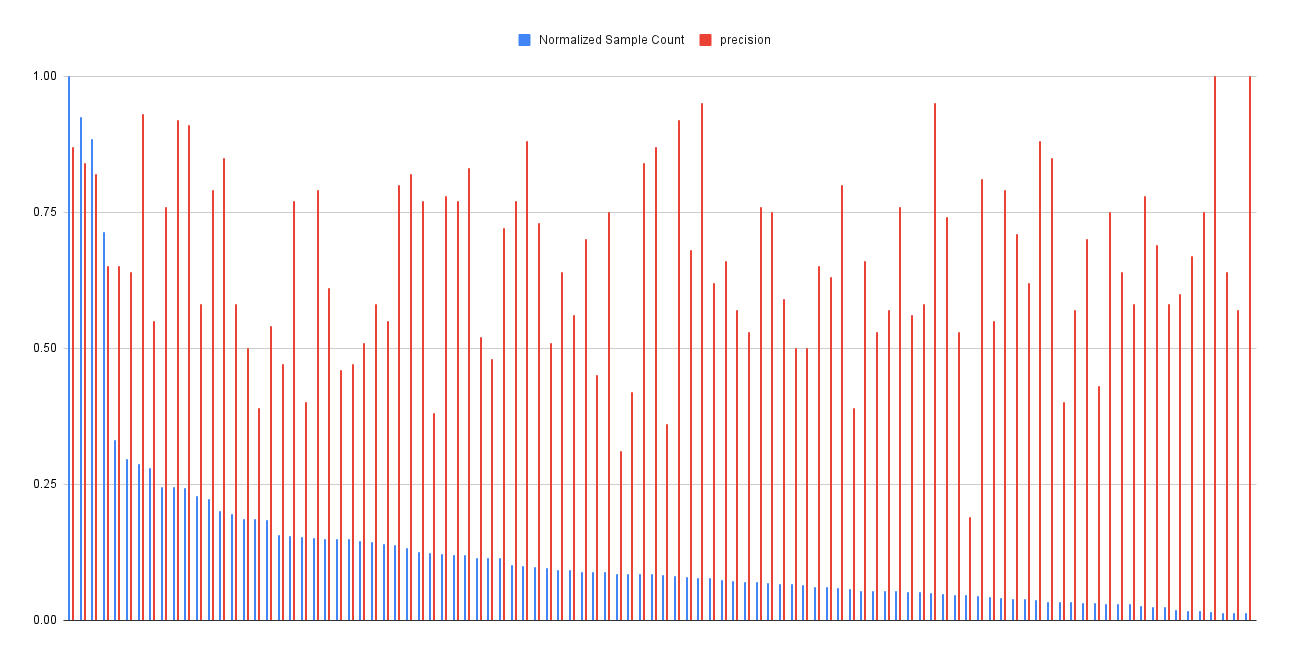
\includegraphics[scale=.5]{figures/chart.png}
    \caption{Precision on ResNet50}
    \label{fig:rn50}
\end{sidewaysfigure}
\begin{sidewaysfigure}
    \centering
    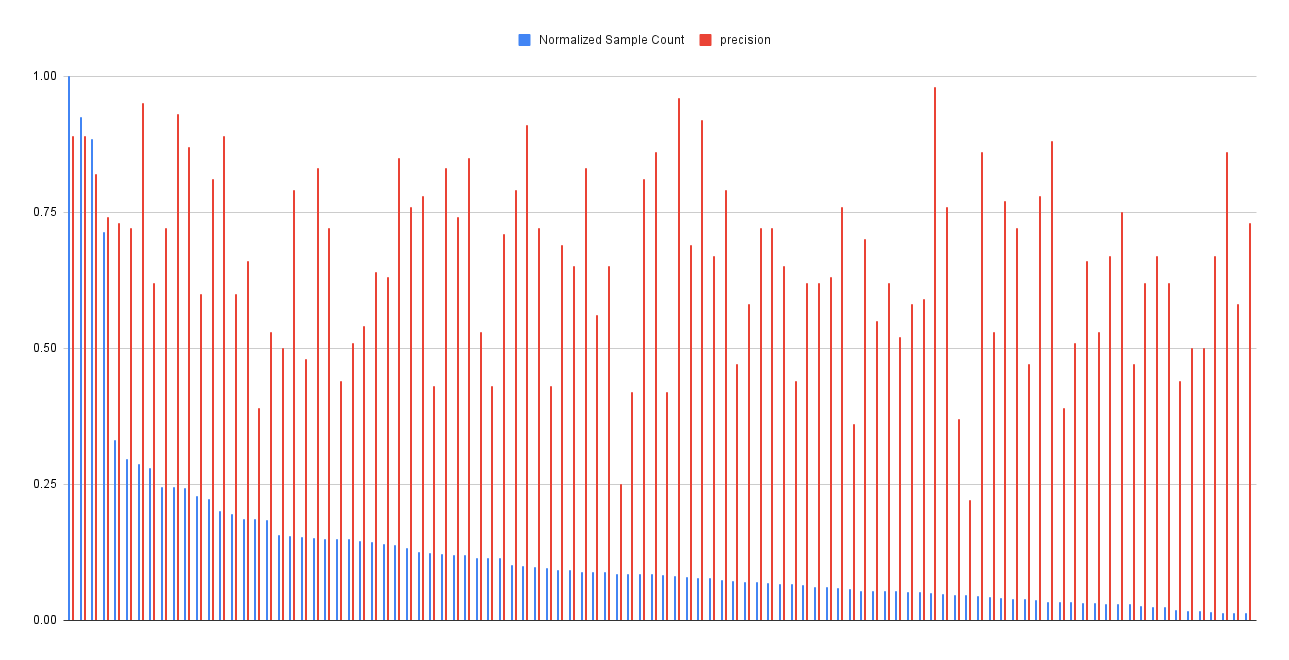
\includegraphics[scale=.5]{figures/chart (1).png}
    \caption{Precision on ResNet152}
    \label{fig:rn152}
\end{sidewaysfigure}
\begin{sidewaysfigure}
    \centering
    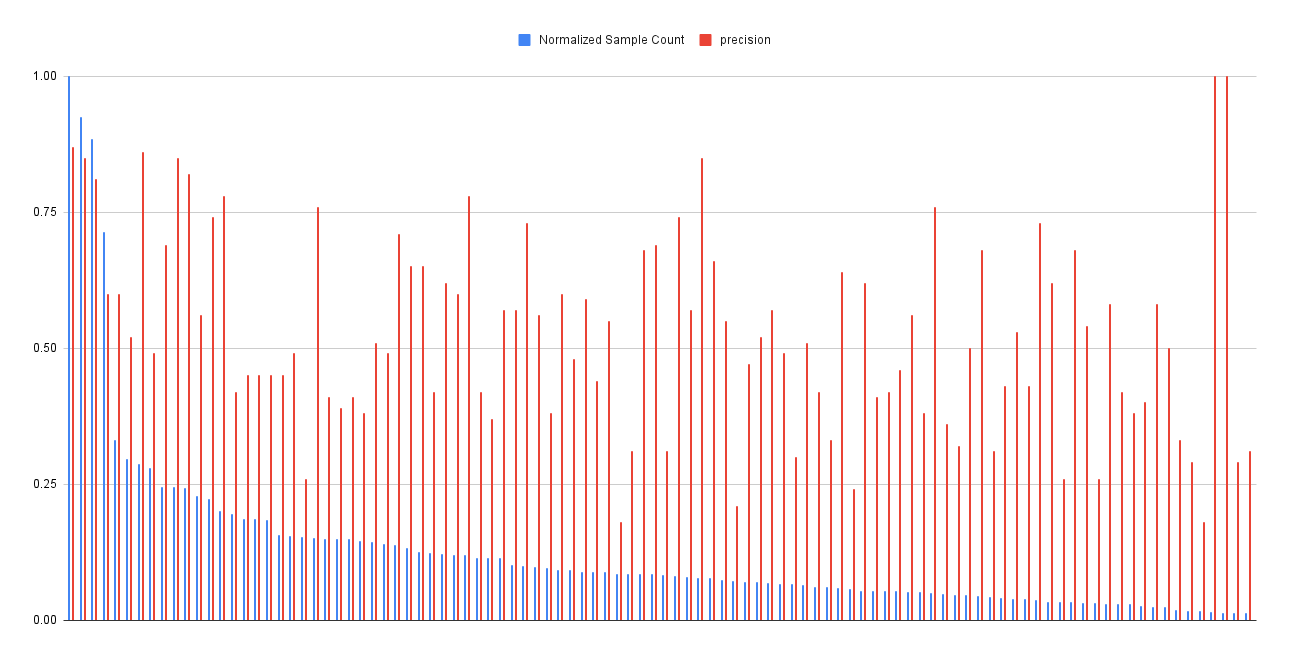
\includegraphics[scale=.5]{figures/chart (2).png}
    \caption{Precision on ResNet18}
    \label{fig:rn18}
\end{sidewaysfigure}


\subsection{Performance of Transfer learning and Fine Tuning}
To classify insect pests, several advanced deep CNN models were used. These models were initially trained on the ImageNet dataset and then fine-tuned using samples of pests from the IP102 dataset. The advantage of this was that the models were already able to recognize intricate patterns, allowing for quicker convergence. The aim was to choose the most appropriate models for the proposed method, so only the final layer of the classifier, which corresponds to classes number in the dataset, was altered.
\begin{sidewaysfigure}
    \centering
    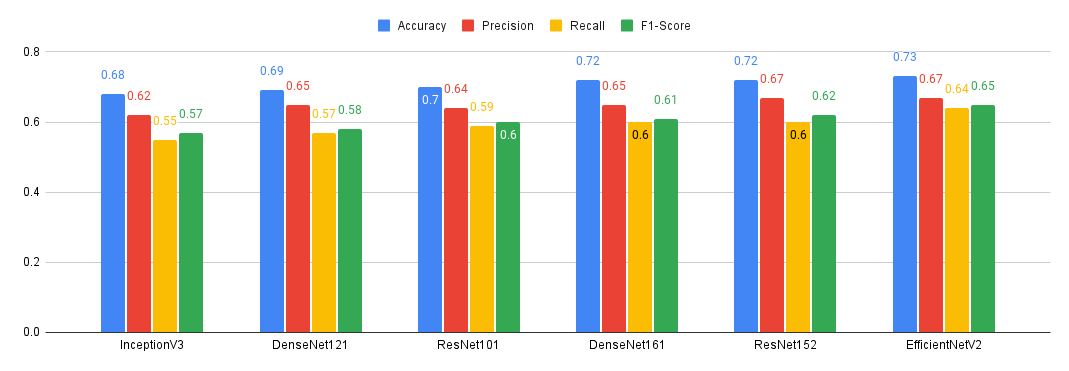
\includegraphics[scale=.7]{figures/chart (3).png}
    \caption{Result of pretrained models on IP102 using Transfer Learning and Augmentation}
    \label{fig:transfer_learning}
\end{sidewaysfigure}


As for the experiment we have used eight pretrained models. For this we prepared all of the models separately. We have used early stopping. The training was stopped if there was no significant change for consecutive 10 epochs for the validation set. Each model was evaluated on the test set of IP102 dataset based on the metrics included in the fig \pageref{fig:transfer_learning}.

The main problem with deeper architectures is that the path for information from input layer to output layer and for the gradient in the opposite direction becomes so long that they face vanishing gradient problem. so each of the models is tackling the issue differently. An inception module consists of multiple convolution and a max pooling operation. using inception module inceptionV3 achieves 68.73\% accuracy. DenseNet and ResNet are very similar with some fundamental differences. ResNet only uses one prior feature-map while DenseNet uses features from all previous convolutional blocks, despite the fact that they both link to the feature-maps of all preceding convolutional blocks.   It reflects on the result too. DeneNet121 and ResNet101 achieve 69.54\% and 70\% respectively. As we can see DenseNet161 and ResNet152 achieve almost the same accuracy of 72\%. So it indicates that the deeper model is doing better on IP102 as there are many variations in the dataset. As the insects are very small in proportion in the images so we opted for attention based pretrained models such as ViT and ConvNext. ConvNext adopted all the training methodologies and architecture design changes introduced by Vision Transformer models. A resNet50 was transformed into ConvNext using those changes. so ConvNext combines the best of the both CNN and transformer world. ConvNext outperforms Vision Transformer(ViT) by a little margin. ConvNext achieves 76\% where ViT achieves 75.38\%.

We also evaluated the experiment using another pest dataset called D0. Here is the result.
\begin{table}[!htbp]
\centering
\begin{tabular}{|c|c|c|c|c|c|c|}
\hline
\textbf{Model} & \textbf{Accuracy} & \textbf{Precision} & \textbf{Recall} & \textbf{F1-Score}\\
\hline
ResNet152 & 0.9840 & 0.9818 & 0.9817 & 0.9807\\
\hline
EfficientNetV2 & 0.9893 & 0.9940 & 0.9925 & 0.9930\\
\hline
ViT & 0.9947 & 0.9962 & 0.994 & 0.9940\\
\hline
ConvNext & 0.7600 & 0.9937 & 0.98170 & 0.9930\\
\hline
\end{tabular}
\caption{Result of pretrained models on D0 dataset using Transfer Learning and Augmentation}
\end{table}


\subsection{Attention Mechanism}
As discussed in the methodology section, we implemented the literature on attention mechanisms in CNN[28]. Here is the result author of the literature used a pretrained model of ResNet50 by fine tuning last layer which achieved 70.53\% accuracy, RAN, a attention module that helps the networks to decide which location of the image may be focused on , achieved 54.40\% accuracy, FPN, an alternative way to construct a pyramid of features for recognizing recognizing objects with highly variant scales, achieved 72\%, MMAL-Net was able to achieve 72.15\%  which is highest among the other models. Then finally ensemble was done of the each model to get a final result of 72.63\%.\\

\begin{figure}
    \centering
    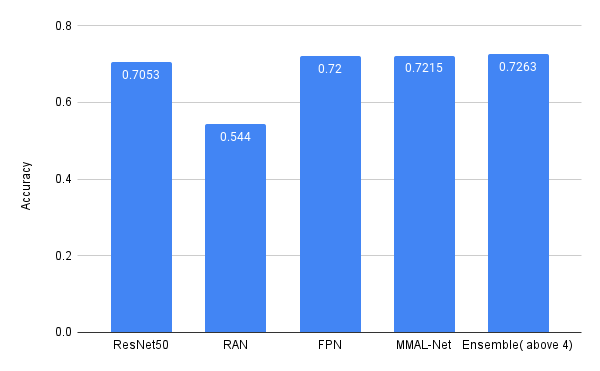
\includegraphics[scale=.65]{figures/chart (4).png}
    \caption{Multiple Conv NN Based Model with Attention}
    \label{fig:my_label}
\end{figure}


We can observe from table 1 that this experiment was not able to perform better than any pretrained model as there are other pretrained models performing better than this.

\subsection{Performance of ensemble model}
We chose four pretrained models based on the result from table 1 which are ResNet, EfficientNetV2, ViT, ConvNext for ensemble using soft voting. We did soft voting of two models as an ensemble of multiple models didn’t provide better results than an ensemble of two models. Here is the table for the ensemble of the pretrained models.\\
\begin{sidewaysfigure}
    \centering
    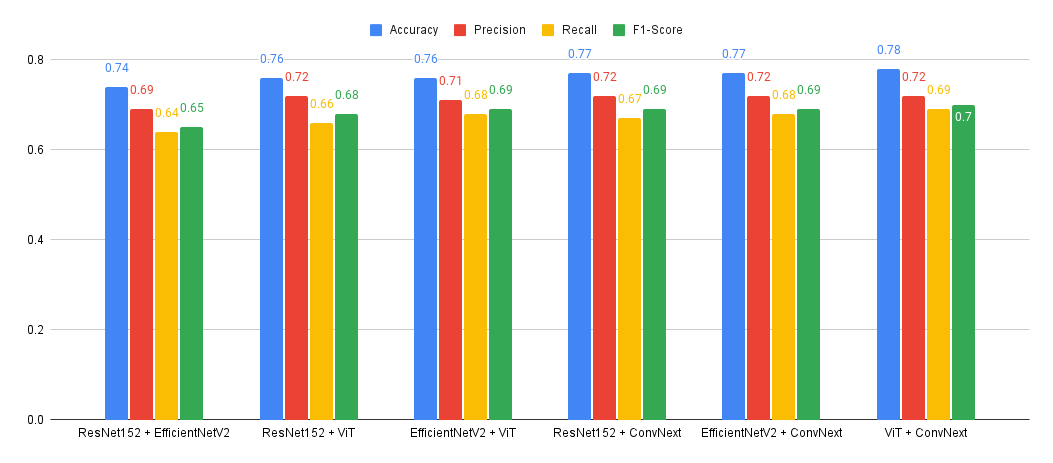
\includegraphics[scale=.7]{figures/chart (5).png}
    \caption{Result of Ensemble of pretrained models on IP102}
    \label{fig:ensemble_result}
\end{sidewaysfigure}

The following observations can be made from the results listed in Table-
\begin{itemize}
    \item Based on overall Accuracy, Precision, Recall and F1- score, the performance of the ensemble of ViT and ConvNext was better than other ensembles. The dataset has the challenges of inter and intra class variance so ensemble of attention based pretrained models did better.
    \item Although the ensemble of ConvNext and ViT did best, we prefer the ensemble of ConvNext and EfficientNet for realtime classification because both convNext and ViT are larger models. As accuracy is the main concern till now we propose vit + convnext. The second best performance is from the ensemble of ConvNext and EfficientNetv2. ConvNets offer several inductive biases which makes them well suited for computer task vision e.g translation variance. Further when ConvNets are used in a sliding window manner, the computations are shared making the whole operation efficient.
    \item ViT usually performs better with large datasets as the inductive biases are not hardcoded. It learns by itself from the dataset. But a large dataset is always a challenge. Also it has a major challenge to work with global attention design with quadratic complexity in ViT. The problem compounds with higher resolution. ConvNext and EfficientNetV2 shine here being pure CNN models.
\end{itemize}

\subsection{Performance of Region of Interest}
The regions of the pest were extracted for the images of the train set using YOLOv5 then the images were fed into the pipeline for training the model. This experiment was done by using three models named ResNet152, EfficientNetV2, ViT. 

From the observation of table 5 and 6 we can conclude that cropping train or train-val didn’t help to improve. The previous results before cropping were better in every case. The reason can be that when the image was cropped from the original image, it was losing information which might be important to the models such as background etc.
\begin{table}[!htbp]
\centering
\begin{tabular}{|c|c|c|c|}
\hline
\textbf{Dataset} & \textbf{Model} & \textbf{Accuracy} & \textbf{Prv (without crop)}\\
\hline
IP102 & EfficientNetV2 & 0.7223 & 0.7315\\
\hline
\end{tabular}
\caption{Result of the experiment using cropped train set only on IP102}
\end{table}


We tried to retrain a model that was already trained on the original dataset using the cropped dataset (train-val) and vice versa.\\
\begin{table}[!htbp]
\centering
\begin{tabular}{|c|c|c|c|}
\hline
\textbf{Dataset} & \textbf{Model} & \textbf{Accuracy} & \textbf{Prv (without crop)}\\
\hline
\multirow{3}{3em}{IP102} & EfficientNetV2 & 0.7173 & 0.7315\\\cline{2-4}
& ResNet152 & 0.6922 & 0.7200\\\cline{2-4}
& VIT & 0.7384 & 0.7538\\\cline{2-4}
\hline
\end{tabular}
\caption{Result of the experiment using cropped train-val-test set on IP102}
\end{table}

Our hypothesis was that retraining an already trained model would be able to fetch more relevant information which can boost the accuracy of the models. But it wasn’t the case. The trained model on the original dataset or cropped dataset wasn’t able to fetch any new information as there were some critical image(those can’t be identified with bare eyes). Those needed to be discarded.
\begin{table}[!htbp]
\centering
\begin{tabular}{|p{0.3\linewidth}|c|c|c|}
\hline
\textbf{Model} & \textbf{Accuracy} & \textbf{Prev (without crop)}\\
\hline
ResNet152 & 0.7000 & 0.7200\\
\hline
ResNet152 & 0.7178 & 0.7200\\
\hline
\end{tabular}
\caption{Retrain ResNet152 using both cropped and original dataset of IP102}
\end{table}



\subsubsection{Performance of STEGO}
We previously segmented our dataset with an unsupervised segmentation technique offered by Hamilton et al.\cite{hamilton2022unsupervised}. The accuracy we got from the train dataset was disappointing as it was not up to the mark.
\begin{table}[!htbp]
\centering
\begin{tabular}{|p{0.3\linewidth}|c|c|c|c|}
\hline
\textbf{Method} & \textbf{Dataset} & \textbf{Model} & \textbf{Accuracy} & \textbf{Prev}\\
\hline
Segmented dataset(train) + Transfer Learning & IP102 & EfficientNetV2 & 0.5896 & 0.7315\\
\hline
\end{tabular}
\caption{Result of the experiment using segmented train set only on IP102}
\end{table}

\begin{sidewaysfigure}
    \centering
    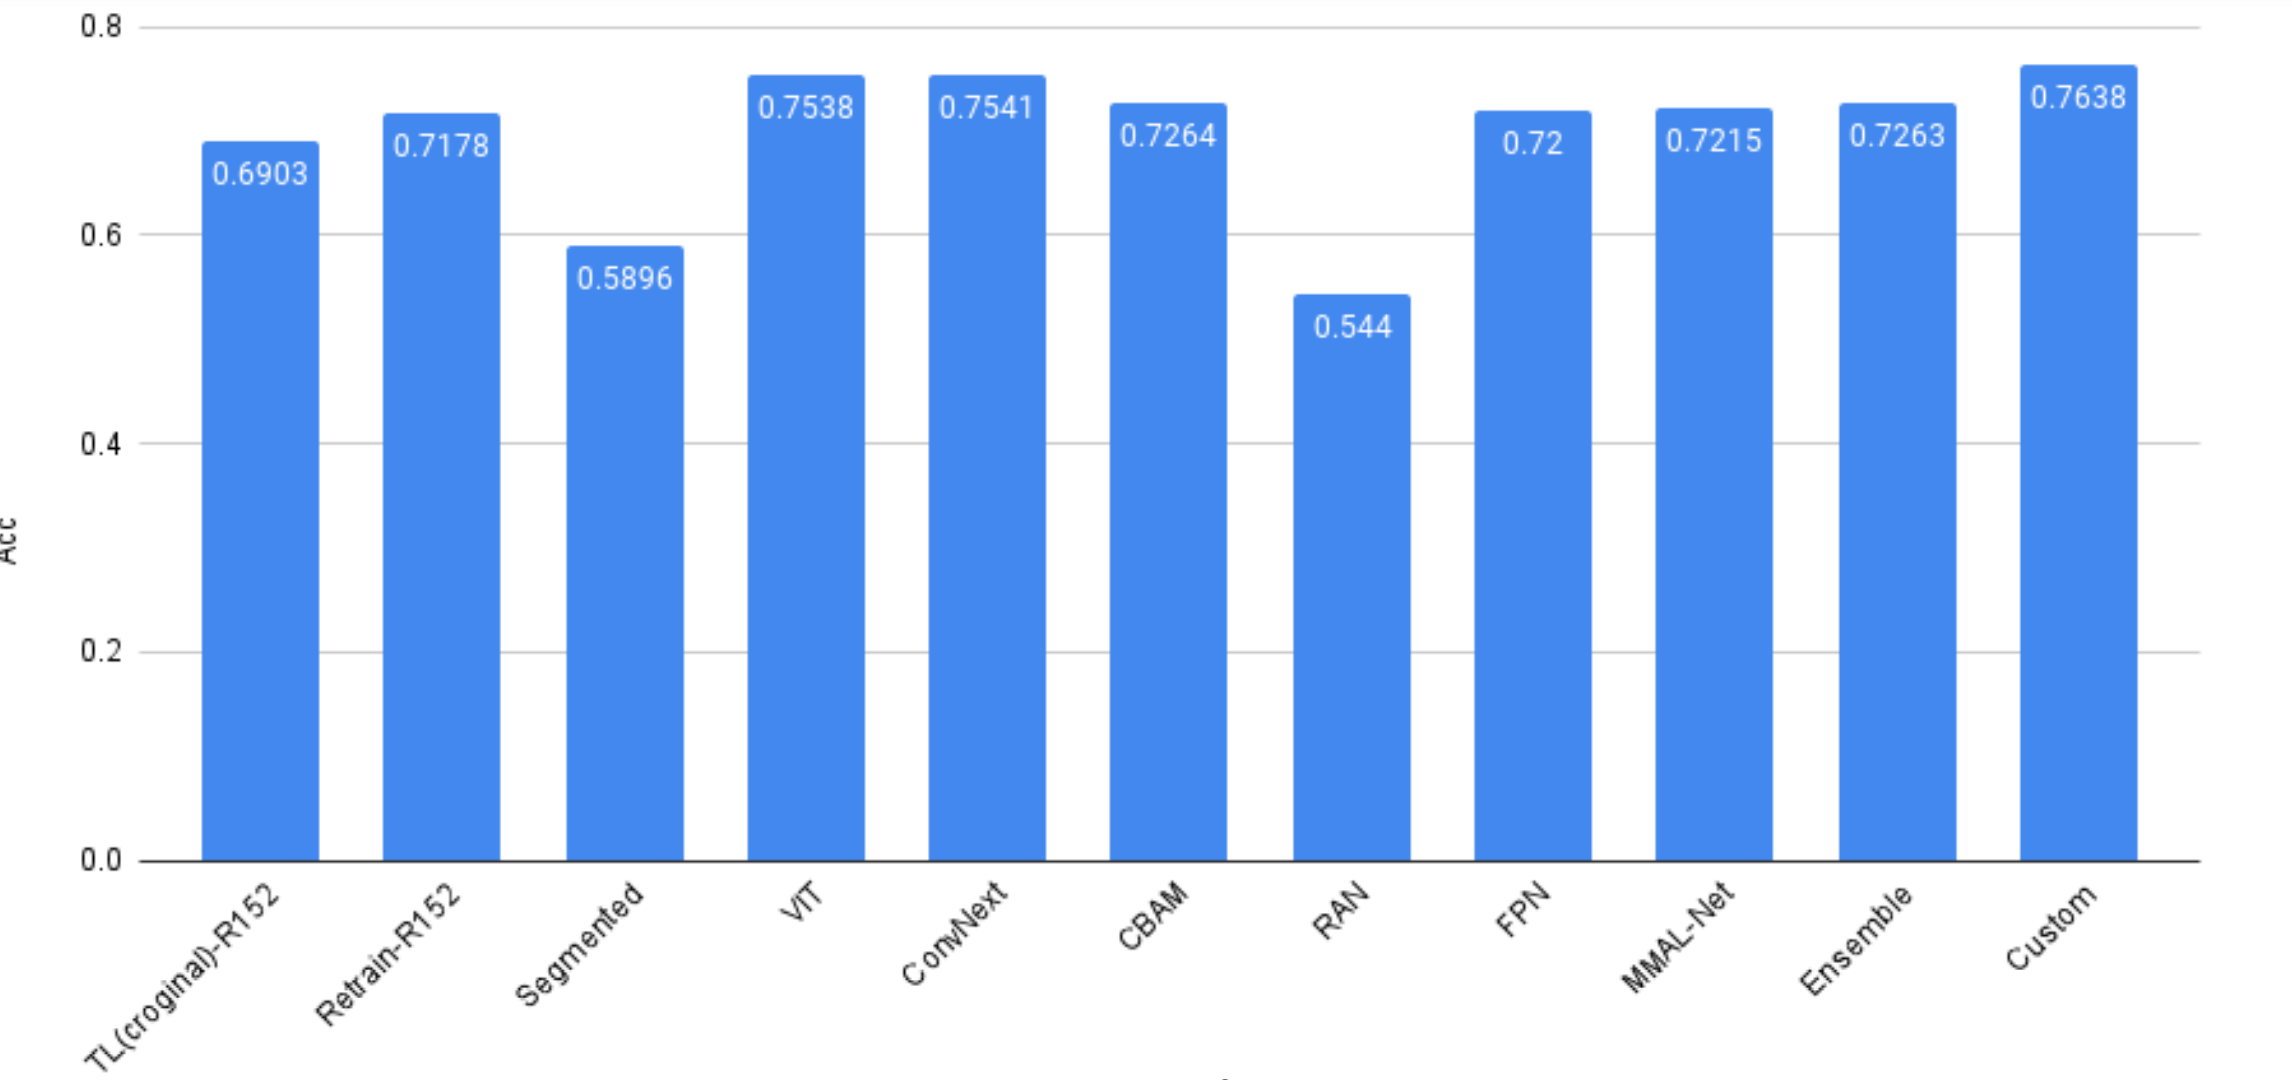
\includegraphics[scale=.5]{figures/Screenshot 2023-05-19 at 4.57.16 AM.png}
    \caption{Result of Focus Region of Interest}
    \label{fig:my_label}
\end{sidewaysfigure}

\subsubsection{Performance of Refined IP102}
As there were many images where either pest is not visible or present, those images were discarded from the whole dataset including train-val-test. Then we performed the transfer learning+fine tuning on the refined dataset to observe the change.
\begin{table}[!htbp]
\centering
\begin{tabular}{|c|c|c|c|c|}
\hline
\textbf{Dataset (train)} & \textbf{Model} & \textbf{Accuracy} & \textbf{Prev (original)}\\
\hline
Changed & \multirow{2}{5em}{ResNet152} & 0.7744 & 0.7200\\\cline{1-1} \cline{3-4}
Unchanged & & 0.5160 & 0.7200\\\cline{1-4}
Changed & \multirow{2}{5em}{ConvNext} & 0.8382 & 0.7600 \\\cline{1-1} \cline{3-4}
Unchanged & & 0.6400 & 0.7600\\
\hline
\end{tabular}
\caption{Performance of Refined IP102 created by Discarding images that do not include pest }
\end{table}
When the images with no pest were discarded from the dataset, it improved the overall accuracy by 5~7\% which is a major improvement. This is the case when the test set is changed with the only yolov5 identified image with 0.5 confidence but if we kept the test set original then the accuracy dropped drastically. This happened because there are some categories of images present in the test set that are not available in the train set. so the model couldn’t generalize properly.
\begin{table}[!htbp]
\centering
\begin{tabular}{|c|c|c|c|}
\hline
\textbf{Reference} & \textbf{Accuracy} & \textbf{F1-Score}\\
\hline
Wu et al.\cite{wu2019ip102} & 0.49 & 0.401\\
Ren et al.\cite{ren2019feature} & 0.5524 & 0.5418\\
Zhou and Su\cite{zhou2020efficient} & 0.5232 & -\\
Nanni et al.\cite{nanni2020insect} & 0.6193 & 0.592\\
Ayan et al.\cite{ayan2020crop} & 0.6713 & 0.6576\\
Yang et al.\cite{yang2021automated} & 0.7329 & -\\
Ung et al.\cite{ung2021efficient} & 0.7413 & 0.6770\\
Nanni et al.\cite{nanni2022high} & 0.7411 & 0.729\\
Peng and Wang\cite{peng2022cnn} & 0.7489 & 0.6814\\
Khan and Ullah\cite{khan2022deep} & 0.8174 & -\\
Li et al.\cite{li2022image} & 0.8650 & 0.8508\\
Our proposed work(Ensemble) & 0.7800 & 0.7056\\
Our proposed Model & 0.8500 & 0.7815\\
\hline
\end{tabular}
\caption{Comparison with Existing works on IP102}
\end{table}
\subsection{Performance of Custom Architecture}
\begin{table}[!htbp]
\centering
\begin{tabular}{|c|c|c|c|c|}
\hline
\textbf{Method} & \textbf{Dataset (train)} & \textbf{Model} & \textbf{Acc} & \textbf{Prev}\\
\hline
\multirow{3}{10em}{Merging the feature extractors + custom classifier} & Changed & \multirow{3}{5em}{ConvNext + ViT} & 0.8500 & 0.7600 \\\cline{2-2}\cline{4-5}
& Unchanged & & 0.6400 & 0.7600\\\cline{2-2}\cline{4-5}
& original dataset & & 0.7638 & 0.7600\\\cline{2-2}\cline{4-5}
\hline
\end{tabular}
\caption{Performance of Custom dataset on both Refined and original IP102}
\end{table}
This time we tried to combine two feature extractor together to extract the information from the images more efficiently. The custom model contains two feature extractors from pretrained models of ViT and ConvNext. We chose these two because of its superior performance on IP102. There is a custom classifier of two fully connected layers, batchnorm1D layers and ReLU activation layers. It showed superior performance on both original and refined IP102 dataset.\\
In refined IP102 the custom model was able to achieve 85\% but 64\% when the original test set was kept. It achieved 76.38\% accuracy when trained on the original IP102 dataset. It performed almost 10\% better than the previous one because unnecessary images were discarded from the dataset which resulted in this much performance improvement.
\begin{table}[!htbp]
\centering
\begin{tabular}{|c|c|c|}
\hline
\textbf{Reference} & \textbf{Accuracy} & \textbf{F1-Score}\\
\hline
Deng et. al \cite{deng2018uav} & 0.8500 & -\\
Xie et al.\cite{xie2015automatic} & 0.8930 & -\\
Thenmozhi and Reddy\cite{thenmozhi2019crop} & 0.9597 & -\\
Dawei et al.\cite{dawei2019recognition} & 0.9384 & -\\
Nanni et al.\cite{nanni2022high} & 0.9553 & -\\
Hazafa et al.\cite{hazafa2022evaluation} & 1.00 & 1.00\\
Our proposed work & 0.9970 & 0.9966\\
\hline
\end{tabular}
\caption{Comparison with Existing works on D0}
\end{table}
\subsection{Performance comparison with existing works}
Finally we have compared our work with existing other literatures. We standout with a accuracy of more than 78\% with ensemble method and our proposed model achieved a highest of 85\% accuracy in IP102 dataset.

We've also compared our work in D0 dataset and it stands out with a 99.7\% accuracy which is the highest after Hazafa et al.'s \cite{hazafa2022evaluation} work.